% !TeX root = bagrut-806.tex

\selectlanguage{hebrew}

\chapter{חדו"א שאלה 
$8$}

%%%%%%%%%%%%%%%%%%%%%%%%%%%%%%%%%%%%%%%%%%%%%%%%%%%%%%%%%%%%%%%%%%%%%%

\section{קיץ תשע"ח מועד ב}

\begin{center}
\selectlanguage{english}
\includegraphics[width=\textwidth]{summer-2018b-8}
\end{center}

\begin{center}
\selectlanguage{english}
\begin{tikzpicture}[scale=1.2]
\clip (0,0) rectangle +(5,4);
\begin{axis}[
    axis lines=center,
    xmin = -.5,
    xmax = 8,
    ymin = -.6,
    ymax = 6,
    xmajorticks=false,
    ymajorticks=false,
]
\addplot [
    domain=.2:6,
    samples=40,
]
{4*(1/x^2)};
\coordinate (A) at (axis cs:1.5,1.78);
\fill (A) circle (1.5pt);
\coordinate (B) at (axis cs:1.5,0);
\fill (B) circle (1.5pt) node[below] {$X$};
\draw (axis cs:0,1.78) -- (axis cs:4,1.78) -- (axis cs:4,0);
\draw[thick,dashed] (A) -- (axis cs:1.5,0);
\path (axis cs:0,0) -- node[left] {$\disfrac{4}{a}$} (axis cs:0,1.78);
\path (axis cs:0,0) -- node[below right] {$a-a'$} (axis cs:4,0);
\path (axis cs:0,0) -- node[below] {$a'$} (axis cs:1.5,0);
\end{axis}
\end{tikzpicture}
\end{center}


\vspace{-2ex}

\textbf{סעיף א}

נתון שהשטח של המלבן הוא
$4$
ולכן הצלע האנכית שלו היא
$\frac{4}{a}$.
נסמן ב-%
$X$
נקודה על ציר ה-%
$x$,
ונסמן את האורך בין
$X$
למרכז הצירים ב-% 
$a'$.
לפי ההגדרה של הפונקציה
$f(a')=\frac{1}{(a')^2}=\frac{4}{a}$
ו-%
$a'=\frac{\sqrt{a}}{2}$.
נחשב את השטח המבוקש כסכום השטח של המלבן עד הנקודה
$X$
והשטח מתחת לפונקציה מ-%
$X$
ועד ל-%
$x=a$:
\erh{14pt}
\begin{equationarray*}{rcl}
S&=&\frac{4}{a}\cdot \frac{\sqrt{a}}{2} + \int_{\frac{\sqrt{a}}{2}}^a \frac{1}{x^2} dx\\
&=&\frac{2}{\sqrt{a}} + \left.(-1)\cdot x^{-1}\right|^a_{\frac{\sqrt{a}}{2}}\\
&=&\frac{2}{\sqrt{a}} - \frac{1}{a} + \frac{1}{\frac{\sqrt{a}}{2}}=\frac{4\sqrt{a}-1}{a}\,.
\end{equationarray*}

\np
\textbf{סעיף ב}

ברור ש-%
$S=\frac{4\sqrt{a}-1}{a}$
יורדת בעיקביות ככל ש-%
$a$
עולה, לכן הערך המקסימלי צריך להיות בערך הקטן ביותר של התחום הנתון
$a=\frac{1}{4}$.
אם רוצים ניתן לחשב את הנגזרת הראשונה:
\[
\left(\frac{4\sqrt{a}-1}{a}\right)'=\frac{\left(4\cdot\frac{1}{2}\cdot a^{-\frac{1}{2}}\cdot a\right) - ((4\sqrt{a}-1)\cdot 1)}{a^2}=\frac{-2\sqrt{a}+1}{a^2}\,,
\]
שמתאפסת ב-%
$a=\frac{1}{4}$.

\np

%%%%%%%%%%%%%%%%%%%%%%%%%%%%%%%%%%%%%%%%%%%%%%%%%%%%%%%%%%%%%%%%%%%%%%

\section{קיץ תשע"ח מועד א}

\begin{center}
\selectlanguage{english}
\includegraphics[width=\textwidth]{summer-2018a-8}
\end{center}

\vspace{-2ex}

\begin{center}
\selectlanguage{english}
\begin{tikzpicture}[scale=.65]
\coordinate (D) at (0,0);
\node[below left] at (D) {$D$};
\coordinate (C) at (6,0);
\node[below right] at (C) {$C$};
\coordinate (A) at (0,6);
\node[above left] at (A) {$A$};
\coordinate (B) at (6,6);
\node[above right] at (B) {$B$};
\draw (A) -- (B) -- node[right] {$6$} (C) -- node[below] {$6$} (D) -- cycle;
\path (A) -- node[left] {$6$} (D);
\coordinate (E) at (2,9);
\node[above] at (E) {$E$};
\draw (D) -- (E) -- (C);
\path[name path=ab] (A) -- (B);
\path[name path=de] (D) -- (E);
\path[name path=cd] (C) -- (E);
\path[name intersections={of=ab and de,by={L}}];
\path[name intersections={of=ab and cd,by={K}}];
\fill (L) circle(1.5pt) node[above left] {$L$};
\fill (K) circle(1.5pt) node[above right] {$K$};
\path (L) -- node[below] {$x$} (K);
\coordinate (F) at ($(D)!(E)!(C)$);
\draw[thick,dashed] (E) -- (F);
\fill (F) circle(1.5pt) node[below] {$F$};
\draw[rotate=90] (F) rectangle +(7pt,7pt);
\coordinate (M) at ($(A)!(E)!(B)$);
\fill (M) circle(1.5pt) node[above right] {$M$};
\draw[rotate=90] (M) rectangle +(7pt,7pt);
\path (E) -- node[right] {$h$} (M);
\end{tikzpicture}
\end{center}

\vspace{-3ex}

\textbf{סעיף א}

לאחר שנשלים סימונים בתרשים, אנו רואים ש-%
$\triangle CDE \sim \triangle KLE$
כי 
$DC \| LK$.
בנוסף, נשים לב שהגובה של
$\triangle CDE$
הוא
$h+6$.
לכן:
\erh{12pt}
\begin{equationarray*}{rcl}
\frac{h}{x}&=&\frac{h+6}{6}\\
h&=&\frac{6x}{6-x}\,.
\end{equationarray*}

\vspace{-4ex}

\textbf{סעיף ב}

נחשב את שלושת השטחים:
\erh{12pt}
\begin{equationarray*}{rcl}
S_{\triangle KLE}&=&\frac{1}{2}\cdot x \cdot h = \frac{1}{2}\cdot x \cdot \frac{6x}{6-x}\\
S_{\triangle ADL}&=&\frac{1}{2}\cdot AL \cdot 6\\
S_{\triangle BCK}&=&\frac{1}{2}\cdot BK \cdot 6\,.
\end{equationarray*}

\np

המצב נראה אבוד כי
$AL,BK$
לא ידועים ואין נתונים עליהם. אבל, נשים לב ש-%
$AB$
היא צלע של הריבוע ולכן
$AL+BK=AB-LK=6-x$.
לכן סכום השטחי המשולשים הוא:
\erh{12pt}
\begin{equationarray*}{rcl}
S=S_{\triangle KLE}+S_{\triangle ADL}+S_{\triangle BCK}&=&
\frac{1}{2}\cdot x \cdot \frac{6x}{6-x}+\frac{1}{2}\cdot (6-x) \cdot 6\\
&=&6\cdot\frac{1}{2} \left(\frac{2(x^2-6x+18)}{6-x}\right)\,.
\end{equationarray*}
נחשב את נגזרת הראשונה )ללא הקבועים
$2$, $\frac{1}{2}$, $6$(:
\erh{12pt}
\begin{equationarray*}{rcl}
S'&=&\frac{(2x-6)(6-x)-(x^2-6x+18)(-1)}{(6-x)^2}\\
&=&\frac{-x^2+12x-18}{(6-x)^2}\,.
\end{equationarray*}
המכנה חיובי ולכן המונה מתאפס עבור:
\[
x=\frac{-12\pm\sqrt{144-4\cdot 18}}{-2}=6\mp 3\sqrt{2}\,.
\]
הערך
$6+3\sqrt{2}>6$
אינו פתרון כי 
$LK$
הוא קטע של צלע שאורכה
$6$.
נקודת הקיצון היא
$6-3\sqrt{2}$.

המכנה של
$S'$
חיובי לכן הסימן של הנגזרת השנייה יהיה הסימן של הנגזרת של המונה של
$S'$
עבור נקודת הקיצון. הנגזרת היא
$-2x+12$.
עבור נקודת הקיצון:
\[
-2(6-3\sqrt{2})+12=6\sqrt{2}>0\,,
\]
והנקודה היא מינימום.

\np

%%%%%%%%%%%%%%%%%%%%%%%%%%%%%%%%%%%%%%%%%%%%%%%%%%%%%%%%%%%%%%%%%%%%%%

\section{חורף תשע"ח}

\begin{center}
\selectlanguage{english}
\includegraphics[width=\textwidth]{winter-2018-8}

\end{center}

\vspace{-1ex}

אני מודה שהסתבכתי כאן בגלל שלא תירגלי מזמן את המשוואה לקו ישר. נדמה לי שזו הפעם היחידה שהמשוואה נדרשת בכל הבחינות הללי.

\textbf{סעיף א}

ערך ההפונקציה חיובית עבור ערכי
$x$
חיוביים, ולכן המשיק נמצא ברביע הראשון.

)הערכים בציר ה-%
$y$
בתרשים הוכפלו פי שמונה כדי לאפשר הצגת תרשים ברור.(

\begin{center}
\selectlanguage{english}
\begin{tikzpicture}%[scale=.8]
\begin{axis}[
    axis lines=center,
    xmin = -.5,
    xmax = 5,
    ymin = -.7,
    ymax = 8,
    ymajorticks=false,
]
\addplot [
    domain=1:5,
    samples=40,
]
{8*(1/x^3)};
\coordinate (A) at (axis cs:2.3,0);
\coordinate (B) at (axis cs:0,6.16);
\coordinate (T) at (axis cs:1.732,1.54);
\fill (A) circle (1.5pt) node[below right] {$A$};
\fill (B) circle (1.5pt) node[left] {$B$};
\fill (T) circle (1.5pt) node[above right] {$\left(t,\disfrac{1}{t^3}\right)$};
\draw[thick,dashed] (T) -- (T|-A) node[below] {$t$};
\draw (A) -- (B);
\fill  (axis cs:0,0)  circle (1.5pt) node[below left] {$O$};
\end{axis}
\end{tikzpicture}
\end{center}

הנגזרת של הפונקציה היא
$f'(x)=\disfrac{-3}{x^4}$
לכן הקו המשיק לגרף הפונקציה הוא:
\[
y-\frac{1}{t^3} = \disfrac{-3}{t^4}(x-t)\,.
\]
נחשב את הנקודות על הצירים:
\erh{12pt}
\begin{equationarray*}{rcl}
0-\frac{1}{t^3} &=& \disfrac{-3}{t^4}(x_A-t)\\
x_A&=&\frac{t}{3}+t=\frac{4t}{3}\\
y_B-\frac{1}{t^3} &=& \disfrac{-3}{t^4}(0-t)\\
y_B&=&\frac{1}{t^3}+\frac{3}{t^3}=\frac{4}{t^3}\,.
\end{equationarray*}

\np

השאלה מבקשת את נקודת הקיצון של:
\[
g(t)=x_A+x_B=\frac{4t}{3}+\frac{4}{t^3}\,.
\]
הנגזרת הראשונה והנגזרת השנייה הן:
\begin{equationarray*}{rcl}
g'(x)&=&\frac{4}{3}+\frac{-12}{t^4}\\
g''(x)&=&\frac{48}{t^5}\,.
\end{equationarray*}
הנחשב את
$t$
כאשר הנגזרת הראשונה מתאפסת:
\erh{12pt}
\begin{equationarray*}{rcl}
g'(t)&=&\frac{4}{3}+\frac{-12}{t^4}=0\\
t^4&=&\frac{3}{4}\cdot 12=9\\
t&=&\pm \sqrt{3}\,.
\end{equationarray*}

נתון ש-%
$t>0$
ולכן נקודת הקיצון היא
$t=\sqrt{3}$.
הנגזרת השנייה חיובית עבור כל
$t>0$
ולכן נקודת הקיצון היא מינימום.

\textbf{סעיף ב}

אם יש רק נקודת קיצון פנימית אחת שהיא מינימום, אז המקסימום חייב להיות בקצה התחום.

\begin{equationarray*}{rcl}
g(1)&=&\frac{4\cdot 1}{3}+\frac{4}{1^3}=\frac{16}{3}\\
g(5)&=&\frac{4\cdot 5}{3}+\frac{4}{5^3}=\frac{20}{3}+\frac{4}{125}\,.
\end{equationarray*}

ברור ש-%
$g(1)<g(5)$
ולכן המקסימום הוא ב-%
$t=5$.


\np

%%%%%%%%%%%%%%%%%%%%%%%%%%%%%%%%%%%%%%%%%%%%%%%%%%%%%%%%%%%%%%%%%%%%%%

\section{קיץ תשע"ז מועד ב}

\begin{center}
\selectlanguage{english}
\includegraphics[width=\textwidth]{summer-2017b-8}
\end{center}

\vspace{-2ex}

בשאלה זו צירך לשים לב להבדל בין חישוב אינטרגל של פונקציה ובין השימוש באינטגרל לחישוב שטח. בתרשים בשאלה, אם מחשבים אינטגרל מ-%
$0$
ל-%
$2\pi$,
הערכים השליליים עד
$\frac{\pi}{2}$
"מורידים" מערך האינטגרל. כאשר מחשבים את השטח
$S_1+S_2$
התרומה של
$S_1$
חיובית ויש לחשב את האינטגרל של השלילה של הפונצקיה.

\textbf{סעיף א}

הערך של 
$f(x)$
שלילי בין
$0$
ל-%
$\frac{\pi}{2}$
ולכן:
\[
S_1+S_2=\int_0^{\frac{\pi}{2}} -f(x) dx + \int_\frac{\pi}{2}^{2\pi} f(x) dx = 10\pi^2+16\,.
\]
נתון ש:
\[
-S_1+S_2=\int_0^{\frac{\pi}{2}} f(x) dx + \int_\frac{\pi}{2}^{2\pi} f(x) dx=\int_0^{2\pi} f(x) dx =8\pi^2\,.
\]
נחסיר את המשוואה השנייה מהראשונה ונקבל:
\[
S_1=\pi^2+8\,.
\]

\np

\textbf{סעיף ב}

\[
-S_1=\int_0^{\frac{\pi}{2}} f(x) dx = \left. F\right|_0^{\frac{\pi}{2}}=F\left(\frac{\pi}{2}\right)- F(0)=F\left(\frac{\pi}{2}\right)=-(\pi^2+8)\,.
\]

\textbf{סעיף ג}

נתון 
$f\left(\disfrac{\pi}{2}\right)=0$.
\erh{12pt}
\begin{equationarray*}{rcl}
f(x) &=& \int f'(x) dx= \int (8\sin x + 8) dx\\
&=&-8\cos x + 8x + c\\
f\left(\disfrac{\pi}{2}\right) &=& -8\cos \frac{\pi}{2} + 8\cdot \frac{\pi}{2} + c = 0\\
c&=&-4\pi\\
f(x) &=& -8\cos x + 8x -4\pi\,.
\end{equationarray*}

\np

%%%%%%%%%%%%%%%%%%%%%%%%%%%%%%%%%%%%%%%%%%%%%%%%%%%%%%%%%%%%%%%%%%%%%%

\section{קיץ תשע"ז מועד א}

\begin{center}
\selectlanguage{english}
\includegraphics[width=\textwidth]{summer-2017a-8}
\end{center}

\vspace{-2ex}

\textbf{סעיף א}

נציב את הביטויים הנתונים עבור 
$A,B$
ונקבל שתי משוואת בשני נעלמים
$t,c$
שנוכל לפתור:
\erh{2pt}
\begin{equationarray*}{rcl}
-(2t)^2+2(2t)+c&=&0\\
-(-t)^2+2(-t)+c&=&0\\
t(6t-3)&=&0\\
t&=&2\,.
\end{equationarray*}
פסלנו את הפתרון
$t=0$
כי נתון ש-%
$t>0$.
נחשב את 
$c$:
\erh{2pt}
\begin{equationarray*}{rcl}
-(-2)^2+2(-2)+c&=&0\\
c&=&8\,.
\end{equationarray*}
הפונקציה היא
$f(x)=-x^2+2x+8$.

\textbf{סעיף ב}

נקודת החיתוך של ציר הסימטריה של הפרבולה עם הפונקציה היא נקודת המקסימום של
$f(x)$.
מהנגזרת הראשונה
$f'(x)=-2x+2=0$
מתקבל
$x=1$.

הקודקודים של 
$\triangle KLM$
הם:
\erh{2pt}
\begin{equationarray*}{rcl}
M&=&(1,0)\\
L&=&(x,0)\\
K&=&(x,-x^2+2x+8)\,.
\end{equationarray*}
השטח של
$\triangle KLM$
הוא:
\[
S(x)=\frac{1}{2}(x-1)(-x^2+2x+8)\,,
\]
והגזרת הראשונה היא:
\erh{12pt}
\begin{equationarray*}{rcl}
S'(x)&=&\frac{1}{2}\cdot -3x^2+6x+6\\
&=&-\frac{3}{2}\cdot(x^2-2x-2)\,.
\end{equationarray*}
הנגזרת מתאפסת ב:
\[
x=\frac{2\pm\sqrt{4+4\cdot 2}}{2}=1\pm\sqrt{3}\,.
\]

השטחים מקסימליים כי חישוב הנגזרת השנייה נותן:
\erh{12pt}
\begin{equationarray*}{rcl}
S''(x)&=&-3 (x-1)\\
S''(1+\sqrt{3})&=&-\sqrt{3}<0\,.
\end{equationarray*}
הפתרון
$1+\sqrt{3}$
מתאים למשולש בתרשים.

הפתרון
$1-\sqrt{3}$
מתאים למשולש הסימטרי משמאל ל-%
$M$.
אורך הבסיס יהיה
$1-x$,
הסימנים יתהפכו ונקבל שטח חיובי ומקסימלי.
\begin{quote}
פתרונות אחרים משתמשים במונח "קודקוד הפרבולה". לא נתקלתי בו בספרי לימוד או בבחינות אחרות. עבור פרבולה
$ax^2+bx+c$
ערך ה-%
$x$
של הקודקוד הוא
$\disfrac{-b}{2a}$.
אין צורך לזכור את הנוסחה כי ניתן לשחזור אותה על ידי חישוב הנגזרת:
\erh{12pt}
\begin{equationarray*}{rcl}
f(x)&=&ax^2+bx+c\\
f'(x)&=&2ax+b=0\\
x&=&\frac{-b}{2a}\,.
\end{equationarray*}
\end{quote}

\np

%%%%%%%%%%%%%%%%%%%%%%%%%%%%%%%%%%%%%%%%%%%%%%%%%%%%%%%%%%%%%%%%%%%%%%

\section{חורף תשע"ז}

\begin{center}
\selectlanguage{english}
\includegraphics[width=\textwidth]{winter-2017-8}

\end{center}

\vspace{-2ex}

\textbf{סעיף א}

$(1)$
במקום לחשב את השטח האפור )משימה שנראית די קשה(, נחשב את שטחו כהפרש בין השטח של גזרת המעגל
$BAC$
לבין השטח של המשולש
$\triangle APL$.

שטח הגזרה הוא שישית משטח המעגל כולו
$\disfrac{1}{6}\cdot\pi R^2$.

שטח המשולש הוא מחצית המכפלת הבסיס
$AL$
והגובה
$PL$,
אבל ניתן להביע אותם באמצעות הרדיוס
$AP=R$
והזווית 
$\alpha=\angle PAC$:
\erh{12pt}
\begin{equationarray*}{rcl}
\cos \alpha &=& \frac{AL}{R}\\
\sin \alpha &=& \frac{PL}{R}\\
S_{\triangle APL}&=&\frac{1}{2}\cdot R\cos \alpha \cdot R\sin \alpha\,.
\end{equationarray*}
השטח האפור הוא:
\[
S_{\textrm{\R{אפור}}} = \frac{R^2}{2}\left(\frac{\pi}{3} - \cos \alpha\sin\alpha\right)
\]
בלי הקבוע
$\frac{R^2}{2}$
הנגזרת הראשונה היא:
\[
-((-\sin \alpha)\cdot \sin\alpha + \cos\alpha\cdot\cos \alpha)=\sin^2 \alpha - \cos^2\alpha\,.
\]
הנגזרת מתאפסת כאשר
$\cos\alpha=\pm\sin\alpha$.
בגזרה
$0<\alpha<\frac{1}{6}\cdot 2\pi$,
הפתרון היחיד הוא
$\alpha=\frac{\pi}{4}$.

\np

$(2)$
הנגזרת השנייה היא
$4\sin\alpha\cos\alpha$
שהיא חיובית בגזרה, ולכן נקודות הקיצון היא מינימום.

נשווה את החישוב שקיבלנו עם השטח הנתון:
\erh{14pt}
\begin{equationarray*}{rcl}
\frac{R^2}{2}\left(\frac{\pi}{3} - \cos \frac{\pi}{4}\sin\frac{\pi}{4}\right)&=&24\pi-36=12(2\pi-3)\\
R^2\left(\frac{\pi}{3} - \frac{\sqrt{2}}{2}\cdot \frac{\sqrt{2}}{2}\right)&=&24(2\pi-3)\\
\frac{R^2}{6}\left(2\pi - 3\right)&=&24(2\pi-3)\\
R&=&12\,.
\end{equationarray*}

\textbf{סעיף ב}

השטח המקסימלי של 
$\triangle APL$
הוא שטח הגזרה פחות השטח המינימלי של השטח האפור:
\erh{12pt}
\begin{equationarray*}{rcl}
S_{\triangle APL}&=&\frac{\pi R^2}{6} - (24\pi - 36)\\
&=&24\pi - (24\pi-36) = 36\,.
\end{equationarray*}

\np

%%%%%%%%%%%%%%%%%%%%%%%%%%%%%%%%%%%%%%%%%%%%%%%%%%%%%%%%%%%%%%%%%%%%%%

\section{קיץ תשע"ו מועד ב}

\begin{center}
\selectlanguage{english}
\includegraphics[width=\textwidth]{summer-2016b-8}

\end{center}


ביזבזתי הרבה זמן על השאלה כי בהעדר תרשים שמתי את הנקודה 
$D$
על היתר 
$AC$!


\begin{center}
\selectlanguage{english}
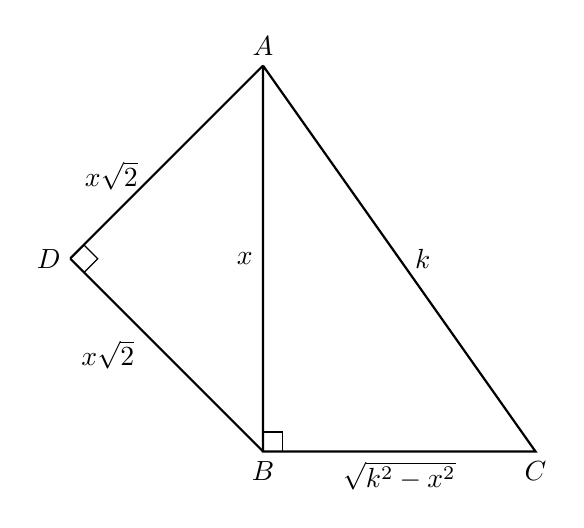
\begin{tikzpicture}[scale=2]
\coordinate (B) at (0,0);
\node[below] at (B) {$B$};
\coordinate (A) at (0,2.45);
\node[above] at (A) {$A$};
\coordinate (C) at (1.73,0);
\node[below] at (C) {$C$};
\draw[thick] (A) -- node[left] {$x$} (B) -- node[below] {$\sqrt{k^2-x^2}$} (C) -- node[right,xshift=2pt] {$k$} (A);
\draw[thick] (B) -- node[left,xshift=-8pt] {$\disfrac{x}{\sqrt{2}}$} +(135:1.73) coordinate (D);
\draw[thick] (A) --  node[above,xshift=-20pt,yshift=-14pt] {$\disfrac{x}{\sqrt{2}}$} +(-135:1.73);
\node[left] at (D) {$D$};
\draw (B) rectangle +(3.5pt,3.5pt);
\draw[rotate=-45] (D) rectangle +(3.5pt,3.5pt);
\end{tikzpicture}
\end{center}


\textbf{סעיף א}

הביטויים עבור
$BC,AD,BD$
נובעים ממשפט פתגורס ומהנתון ש-%
$\triangle ADB$
שווה-שוקיים.

\medskip

\textbf{סעיף ב}
\erh{16pt}
\begin{equationarray*}{rcl}
\left(BC\cdot AD^2\right)'&=& \left(\sqrt{k^2-x^2}\cdot \frac{x^2}{2}\right)'\\
&=& \frac{-2x}{2\sqrt{k^2-x^2}}\cdot\frac{x^2}{2}+\sqrt{k^2-x^2}\cdot x\\
&=& \frac{2k^2x-3x^3}{2\sqrt{k^2-x^2}}\,.
\end{equationarray*}
נניח כמובן שהמשולש לא מנוון כך ש-%
$x\neq 0$.
הנגזרת מתאפסת כאשר:
\[
k=\sqrt{\frac{3}{2}}x,\quad\quad x=\sqrt{\frac{2}{3}}k\,.
\]

סימן הנגזרת השנייה הוא סימן הנגזרת של המונה של הנגזרת הראשונה:
\[
(2k^2-3x^2)'=-6x<0\,,
\]
נקודת הקיצון היא מקסימלית.

נחשב
$BC\cdot AD^2 = 3\sqrt{3}$
כדי לקבל ערך מספרי עבור
$k$.
נציב
$x=\sqrt{\frac{2}{3}}k$:
\erh{12pt}
\begin{equationarray*}{rcl}
\sqrt{k^2-x^2}\cdot \frac{x^2}{2}&=&\sqrt{k^2-\frac{2}{3}k^2}\cdot \frac{1}{2}\cdot\frac{2}{3}k^2\\
&=&k^3\sqrt{\frac{1}{3}}\cdot \frac{1}{3}=3\sqrt{3}\\
k^3&=&27\\
k&=&3\,.
\end{equationarray*}
מכאן ש:
\[
x=\sqrt{\frac{2}{3}}k=\sqrt{6}\,.
\]

השטח המקסימלי של
$\triangle ADB$
הוא:
\[
\frac{1}{2}\cdot \frac{x}{\sqrt{2}} \cdot \frac{x}{\sqrt{2}} = \frac{x^2}{4} = \frac{(\sqrt{6})^2}{4}=1.5\,.
\]


\np

%%%%%%%%%%%%%%%%%%%%%%%%%%%%%%%%%%%%%%%%%%%%%%%%%%%%%%%%%%%%%%%%%%%%%%

\section{קיץ תשע"ו מועד א}

\begin{center}
\selectlanguage{english}
\includegraphics[width=\textwidth]{summer-2016a-8a}
\includegraphics[width=\textwidth]{summer-2016a-8b}

\end{center}


השאלה ארוכה מאוד אבל התשובות קצרות!

אני הסתבכתי כי לא פעלתי לפי ההנחייה: "היעזר בגרפים ...".

\np

\textbf{סעיף א}

$f(x)\limit{+\infty} 1$
ויש
\asm{}
אופקית ב-%
$y=1$.
עבור
$x\rightarrow -\infty$,
עדיין יש
\asm{}
אופקית ב-%
$y=0$,
רק 
$f(x)$
שואפת ל-%
$0$
מעל לציר ה-%
$x$
עבור
$n$
זוגית, ומתחת לציר עבור 
$n$
אי-זוגי.

הפונקציה לא מוגדרת עבור
$x=0$
ולכן 
$x=0$
היא
\asm{}
אנכית.

\textbf{סעיף ב}
\erh{6pt}
\begin{equationarray*}{rcl}
f'(x)&=&\left(\left(1+x^{-1}\right)^n\right)'\\
&=&n\left(1+x^{-1}\right)^{n-1}\cdot - x^{-2}\,.
\end{equationarray*}
נתון ש-%
$n$
חיובית. אם 
$n$
אי-זוגית,
$n-1$
זוגית, ו-%
$\left(1+x^{-1}\right)^{n-1}$
חיובית או אפס. כמובן ש-%
$x^{-2}$
חיובית )ולא אפס כי נתון ש-%
$x\neq 0$.
לכן סימן המינוס לפני
$x^{-2}$
גורם לכל הביטוי להיות שלילי.

מכאן שגרף
$I$
מתאים ל-%
$n$
אי-זוגית וגרף
$II$
ל-%
$n$
זוגית.

\textbf{סעיף ג}

$(1)$
בנקודת קיצון של
$f(x)$
הנגזרת הראשונה 
$f'(x)$
\textbf{חוצה}
את ציר ה-%
$x$,
לכן אין נקודות קיצון.

$(2)$
בנקודת פיתול הנגזרת השנייה מתאפסת. זה קורה פעם אחת משמאל למינימום של
$f'(x)$
ופעם אחת כאשר ל-%
$f'(x)$
יש נקודות מקסימום ללא שינוי בסימן. לכן יש שתי נקודות פיתול.

\textbf{סעיף ד}

$(1)$
בנקודת קיצון של
$f(x)$
הנגזרת הראשונה 
$f'(x)$
\textbf{חוצה}
את ציר ה-%
$x$,
לכן יש נקודת קיצון אחת.

$(2)$
נקודת פיתול הנגזרת השנייה מתאפסת, כלומר, יש נקודת קיצון לנגזרת הראשונה, לכן יש נקודת פיתול אחת.


$(3)$
לפי גרף 
$II$,
עבור
$x<0$,
השיפוע קרוב לאפס ב%
\asm{}
האופקית. השיפוע יורד משמאל עד לנקודת פיתול שם השיפוע עולה עד לנקודת מינימום של
$f(x)$,
ואז השיפוע עולה. עבור
$x>0$
השיפוע תמיד עולה מערך שלילי נמוך מאוד ועד קרוב לאפס בכיוון ה%
\asm{}
האופקית.

\begin{center}
\selectlanguage{english}
\begin{tikzpicture}%[scale=.8]
\begin{axis}[
    axis lines=center,
    xmin = -6,
    xmax = 6,
    ymin = -.1,
    ymax = 2,
    xmajorticks=false,
    ymajorticks=false,
]
\addplot [
    domain=-6:-.2,
    samples=40,
]
{(1+(1/x))^2};
\addplot [
    domain=.2:6,
    samples=40,
]
{(1+(1/x))^2};
\fill (axis cs:-1,0) circle(1.5pt);
\draw[thick,dashed] (axis cs:-6,1) -- (axis cs:6,1);
\end{axis}
\end{tikzpicture}
\end{center}


\textbf{סעיף ה}

רואים בשני הגרפים שעבור
$x>0$,
השיפוע, הנגזרת הראשונה, עולה, כך שהנגזרת השנייה חיובית. מכפלה של שני ערכים חיוביים היא חיובית.


\np


%%%%%%%%%%%%%%%%%%%%%%%%%%%%%%%%%%%%%%%%%%%%%%%%%%%%%%%%%%%%%%%%%%%%%%

\section{חורף תשע"ו}

\begin{center}
\selectlanguage{english}
\includegraphics[width=\textwidth]{winter-2016-8}

\end{center}

\vspace{-2ex}


\textbf{סעיף א}

הפונקציה לא מוגדרת כאשר המכנה מתאפס: 
$x=-1$.

ב-%
$x=-1$
יש 
\asm{} 
אנכית כי המכנה מתאפס והמונה לא מתאפס.

$y=1$
היא
\asm{} 
אופקית כי:
\[
\frac{1-\frac{1}{x}}{1+\frac{1}{x}}\limit{\pm \infty} 1\,.
\]

\textbf{סעיף ב}

בתרשים סימנו את ערכי ה-%
$x$
ליד שמות הנקודות:
\begin{center}
\selectlanguage{english}
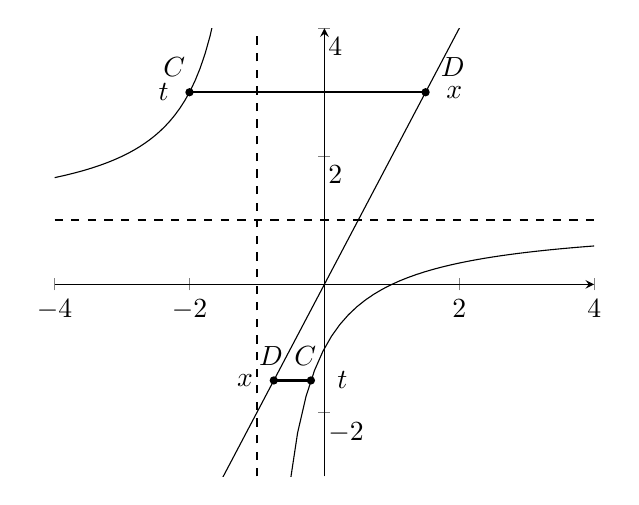
\begin{tikzpicture}%[scale=.8]
\begin{axis}[
    axis lines=center,
    xmin = -4,
    xmax = 4,
    ymin = -3,
    ymax = 4,
    yticklabel style={anchor=north west,},
]
\addplot [
    domain=-4:-1.1,
    samples=40,
]
{(x-1)/(x+1)};
\addplot [
    domain=-.9:4,
    samples=40,
]
{(x-1)/(x+1)};
\addplot [
    domain=-4:4,
    samples=40,
]
{2*x};
\fill (axis cs:-2,3) circle(1.5pt) node[left,xshift=-4pt] {$t$} node[above left,xshift=2pt,yshift=2pt] {$C$};
\fill (axis cs:1.5,3) circle(1.5pt) node[right,xshift=4pt] {$x$} node[above right,xshift=2pt,yshift=2pt] {$D$};
\fill (axis cs:-.2,-1.5) circle(1.5pt) node[right,xshift=6pt] {$t$} node[above,xshift=-2pt,yshift=2pt] {$C$};
\fill (axis cs:-.75,-1.5) circle(1.5pt) node[left,xshift=-4pt] {$x$} node[above,xshift=-1pt,yshift=2pt] {$D$};
\draw[thick] (axis cs:-2,3) -- (axis cs:1.5,3);
\draw[thick] (axis cs:-.75,-1.5) -- (axis cs:-.2,-1.5);
\draw[thick,dashed] (axis cs:-4,1) -- (axis cs:4,1);
\draw[thick,dashed] (axis cs:-1,-3) -- (axis cs:-1,4);
\end{axis}
\end{tikzpicture}
\end{center}

\np

יש כאן מלכודת שניתן להימנע ממנו רק אם מציירים תרשים מדוייק. אמנם
$t$
מוגדר כערך ה-%
$x$
של 
$f(x)$
אבל 
\textbf{האורך}
בין הפונקציה והקו
$y=2x$
תלוי במיקום היחסי בין הקו וגרף הפונקציה. ניתן גם לראות בחלוקה לשני תת-סעיפים רמז שיש לטפל בשני המקרים בנפרד.


$(1)$
כאשר 
$t>-1$
אורך הקטע 
$DC$
)נסמן
$a$(
הוא
$a=-x-(-t)=t-x$.
)מדובר במקרה ש-%
$t,x$
שליליים, אבל הנוסחה מתאימה גם אם קטע הקו במקום אחר.(
ערכי ה-%
$y$
של שתי הנקודות שווים, ולכן ניתן להציב בנוסחה עבור
$a$:
$x=\frac{y}{2}=\frac{f(t)}{2}$:
\erh{12pt}
\begin{equationarray*}{rcl}
a&=&t-x=t-\frac{t-1}{2(t+1)}\\
&=&\frac{2t^2+t+1}{2(t+1)}\\
a'&=&\frac{(4t+1)\cdot 2(t+1) - (2t^2+t+1)(2)}{4(t+1)^2}\\
&=&\frac{4t^2+8t}{4(t+1)^2}=\frac{t(t+2)}{(t+1)^2}=0\,.
\end{equationarray*}

\vspace{-2ex}

ערכי
$t$
של נקודות הקיצון נמצאות במקומות שהנגזרת הראשונה מתאפסת:
$t=0,t=-2$.
המכנה של הנגזרת הראשונה תמיד חיובי ולכן סוג נקודות הקיצון נקבל מהסימן של הנגזרת של המונה:
$2t+2$.
כאשר 
$t=0$,
הנגזרת חיובית והנקודה היא מינימים. כאשר
$t=-2$
הנגזרת שלילית והנקודה היא מקסימום. לכן האורך המינימלי הוא:
\[
t-x=0-\frac{0-1}{2(0+1)}=\frac{1}{2}\,.
\]
$(2)$
כאשר 
$t<-1$
אורך הקטע
$a$
הוא
$a=x+(-t)=x-t$.

\vspace{-4ex}

\erh{12pt}
\begin{equationarray*}{rcl}
a&=&x-t=\frac{t-1}{2(t+1)}-t\\
&=&\frac{-(2t^2+t+1)}{2(t+1)}\\
a'&=&\frac{-(4t+1)\cdot 2(t+1) + (2t^2+t+1)(2)}{4(t+1)^2}\\
&=&\frac{-4t^2-8t}{4(t+1)^2}=\frac{-t(t+2)}{(t+1)^2}=0\,.
\end{equationarray*}
ערכי
$t$
של נקודות הקיצון נמצאות במקומות שהנגזרת הראשונה מתאפסת, שוב ב-%
$t=0, t=-2$.
המכנה של הנגזרת הראשונה תמיד חיובי ולכן סוג נקודות הקיצון מתקבל מהסימן של הנגזרת של המונה:
$-(2t+2)$.
כאשר 
$t=0$,
הנגזרת שלילית והנקודה היא מקסימום. כאשר
$t=-2$
הנגזרת חיובית והנקודה היא מינימום. לכן, האורך המינימלי הוא:
\[
x-t=-\frac{-2-1}{2(-2+1)}-(-2)=\frac{7}{2}\,.
\]
\textbf{סעיף ג}

$\frac{1}{2}<\frac{7}{2}$
לכן האורך המינימלי עבור
$t\neq -1$
הוא
$\frac{1}{2}$
כאשר
$t=0$.


\np

%%%%%%%%%%%%%%%%%%%%%%%%%%%%%%%%%%%%%%%%%%%%%%%%%%%%%%%%%%%%%%%%%%%%%%

\section{קיץ תשע"ה מועד ב}

\begin{center}
\selectlanguage{english}
\includegraphics[width=\textwidth]{summer-2015b-8a}
\includegraphics[width=\textwidth]{summer-2015b-8b}

\end{center}

\vspace{-2ex}

\textbf{סעיף א}

)בשאלה אין נוסחה לפנוקציה, גם לא לאחר פתרון השאלה, ולכן התרשים הוא ממש "סקיצה".(

\begin{center}
\selectlanguage{english}
\begin{tikzpicture}%[scale=.8]
\begin{axis}[
    axis lines=center,
    xmin = 0,
    xmax = 7,
    ymin = -4,
    ymax = 3.2,
    ymajorticks=false,
]
\addplot [
    smooth,
] plot coordinates
{(.1,-4) (.2,-3) (.4,-1.8) (.6,-1) (1,0) (2,2) (3,3) (4,2) (5,1) (6,0.5) (7,0.2)};
\fill (axis cs:1,0) circle(1.5pt);
\fill (axis cs:3,3) circle(1.5pt);
\end{axis}
\end{tikzpicture}
\end{center}

\np

\textbf{סעיף ב}

קיימת נקודת קיצון ב-%
$x=1$
כי הנגזרת הראשונה מתאפסת ומחליפה סימן. הנקודה היא מינימום כי הנגזרת עולה.


\textbf{סעיף ג}

הנגזרת השנייה היא השיפוע של הנגזרת הראשונה, שהוא חיובי עבור
$0<x<3$
ושלילי עבור
$3<x$.
לכן הפונקציה קעורה כלפי מעלה ב-%
$0<x<3$
וקעורה כלפי מטה ב-%
$3<x$.


\textbf{סעיף ד}

אם הפונקציה מקבלת ערכים 
$y\geq 4$
אזי נקודות המינימום שמתקבלת ב-%
$x=1$
צריך לקבל את הערך
$y=4$.
נשתמש בנתון שלפונקציה יש 
\asm{}
ב-%
$x=0$,
וכיווני הקעירות מסעיף ג כדי להשלים את צורת הגרף:

\begin{center}
\selectlanguage{english}
\begin{tikzpicture}%[scale=.8]
\begin{axis}[
    axis lines=center,
    xmin = 0,
    xmax = 7.2,
    ymin = 0,
    ymax = 7.2,
]
\addplot [
    smooth,
] plot coordinates
{(.1,7) (.4,5) (.6,4.5) (1,4) (2,5.2) (3,6) (7,6.3)};
\fill (axis cs:1,4) circle(1.5pt);
\fill (axis cs:3,6) circle(1.5pt);
\end{axis}
\end{tikzpicture}
\end{center}


\textbf{סעיף ה}

$f(x)$
חיובית בכל תחום ההגדרה, לכן גם
$f^3(x)$
חיובית. סימן המינוס הופך את הסימן של ערך הפונקציה. 
$f(x)$
יורד ב-%
$0<x<1$
ולכן 
$g(x)$
עולה בתחום זה.
$f(x)$
עולה ב-%
$1<x$
ולכן 
$g(x)$
יורד בתחום זה.

אפשר להשתמש בנגזרת של
$g(x)$:
\[
g'(x)=-3 f^2(x) f'(x)\,.
\]
$f^2(x)$
תמיד חיובי, ולכן לאור המינוס בתחילת הביטוי, תחומי העלייה והירדה הם התחומים שערכי
$f'(x)$
שליליים או חיוביים בהתאמה.
$f'(x)$
חותך את ציר ה-%
$x$
משליליים לחיוביים ב-%
$x=1$,
ולכן 
$g(x)$
עולה ב-%
$0<x<1$
ויורד ב-%
$1<x$.


\np


%%%%%%%%%%%%%%%%%%%%%%%%%%%%%%%%%%%%%%%%%%%%%%%%%%%%%%%%%%%%%%%%%%%%%%

\section{קיץ תשע"ה מועד א}

\begin{center}
\selectlanguage{english}
\includegraphics[width=.9\textwidth]{summer-2015a-8}
\end{center}

\vspace{-2ex}

\textbf{סעיף א}

נגזרת ראשונה:

\vspace{-5ex}

\erh{10pt}
\begin{equationarray*}{rcl}
f'(x)&=& x^2 -a^2=0\\
x&=&\pm a\\
f''(x)&=&2x\\
f''(+a)&=&2a>0\\
f''(-a)&=&-2a<0\,.
\end{equationarray*}

\vspace{-4ex}

בשתי השורות האחרונות השתמשנו בנתון
$a>0$.

המקסימום הוא ב-%
$x=-a$
והמינימום הוא ב-%
$x=a$.

\textbf{סעיף ב}

המינימום הוא ב-%
$x=a$.
\[
f(a) = -\frac{2}{3}a^3+a^2 = a^2\left(-\frac{2}{3}a+1\right)\,. 
\]
$a^2$
חיובי ולא משפיע על סימן של נקודות המינימום. הפתרון מתקבל על ידי השוואת
$-\frac{2}{3}a+1$
לאפס:
\erh{12pt}
\begin{equationarray*}{rcl}
a&=&\frac{3}{2}\quad\quad\quad$x-$\textrm{\R{על ציר ה}}\\
a&<&\frac{3}{2}\quad\quad\quad$x-$\textrm{\R{מעל ציר ה}}\\
a&>&\frac{3}{2}\quad\quad\quad$x-$\textrm{\R{מתחת לציר ה}}\,.
\end{equationarray*}

\np

\textbf{סעיף ג}

נקודות המינימום מסומנות.

קו רציף: על הציר. קו מקווקוו: מעל לציר. קו מנוקד: מתחת לציר.

\begin{center}
\selectlanguage{english}
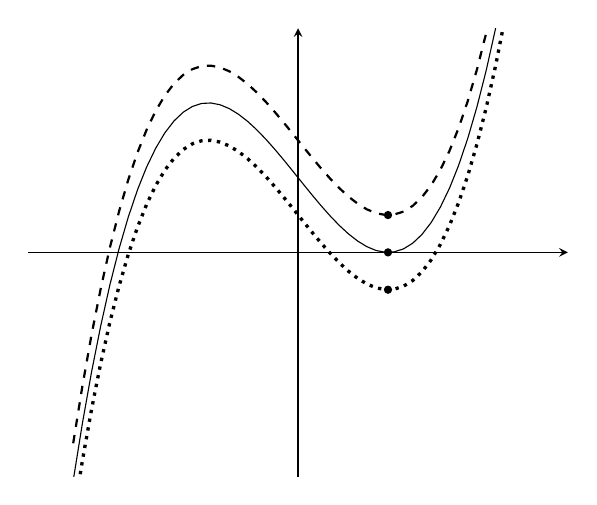
\begin{tikzpicture}%[scale=.8]
\begin{axis}[
    axis lines=center,
    xmin = -3,
    xmax = 3,
    ymin = -2,
    ymax = 2,
    xmajorticks=false,
    ymajorticks=false,
]
\addplot [
    domain=-2.5:2.5,
    samples=50,
]
{.333*x^3-x+1-.333};
\addplot [
    domain=-2.5:2.5,
    samples=50, 
    thick, dashed,
]
{.333*x^3-x+1};
\addplot [
    domain=-2.5:2.5,
    samples=50, 
    very thick, dotted,
]
{.333*x^3-x+1-.666};
\fill (axis cs:1,.333) circle(1.5pt);
\fill (axis cs:1,0) circle(1.5pt);
\fill (axis cs:1,-.333) circle(1.5pt);
\end{axis}
\end{tikzpicture}
\end{center}


\textbf{סעיף ד}

משוואה זו היא המשוואה הנתונה בשאלה כאשר
$a=1$.
אבל 
$1<\frac{3}{2}$,
ולכן לפי סעיף ב המינימום נמצא מעל לציר ה-%
$x$.
מכאן שאין פתרון אחר פרט לנקודת החיתוך של הגרף לפני המקסימום.

\np


%%%%%%%%%%%%%%%%%%%%%%%%%%%%%%%%%%%%%%%%%%%%%%%%%%%%%%%%%%%%%%%%%%%%%%

\section{חורף תשע"ה}

\begin{center}
\selectlanguage{english}
\includegraphics[width=.9\textwidth]{winter-2015-8}
\end{center}

\vspace{-2ex}

\textbf{סעיף א}

לפי הנוסחה לנגזרת של חזקה של פונקציה,
$(f(x)^{\frac{1}{2}})' = \frac{1}{2}f(x)^{-\frac{1}{2}}f'(x)$
שהיא הפונקציה המופיעה באינטגרל. נחשב את ערך האינטגרל:

\vspace{-3ex}

\erh{12pt}
\begin{equationarray*}{rcl}
\int_0^3 \frac{f'(x)}{2\sqrt{f(x)}}\, dx &=& \left. \sqrt{f(x)}\right|_0^3\\
&=&\sqrt{f(3)}-\sqrt{f(0)} = \sqrt{f(3)}-1=3\\
f(3)&=&4^2=16\,.
\end{equationarray*}

\vspace{-3ex}

הפונקציה
$f(x)$
מתקבלת מאינטגרציה של הנוסחה הנתונה לנגזרת ומחישוב הקבוע והפרמטר מהערכים הידועים של
$f(0),f(3)$:
\erh{12pt}
\begin{equationarray*}{rcl}
f(x)&=&\int (kx+2)\,dx = \frac{1}{2}kx^2+2x+c\\
f(0)&=&c=1\\
f(3)&=&\frac{9}{2}k+7=16\\
k&=&2\\
f(x)&=&x^2+2x+1\,.
\end{equationarray*}

\np


\textbf{סעיף ב}

\[
g(x)=\sqrt{f(x)}=\sqrt{x^2+2x+1}=\sqrt{(x+1)^2}=|x+1|\,.
\]
אם
$x\geq -1$,
$x+1$
לא שלילי ו-%
$g(x)=x+1$.

אם 
$x<-1$,
$x+1$
שלילי ו-%
$g(x)=-(x+1)$.

ביחד יש לנו
$g(x)=|x+1|$.


\medskip

\textbf{סעיף ג}

\begin{center}
\selectlanguage{english}
\begin{tikzpicture}%[scale=.8]
\begin{axis}[
    axis lines=center,
    xmin = -3,
    xmax = 3,
    ymin = -1,
    ymax = 2,
]
\addplot [
    domain=-3:2,
    samples=50,
]
{x^2+2*x+1};
\addplot [
    domain=-3:2,
    samples=50,
]
{abs(x+1)};
\fill (axis cs:0,1) circle(1.5pt);
\fill (axis cs:-1,0) circle(1.5pt);
\node at (axis cs: 1,1.5) {$g(x)$};
\node at (axis cs: -1.75,1.5) {$f(x)$};
\end{axis}
\end{tikzpicture}
\end{center}


\np

%%%%%%%%%%%%%%%%%%%%%%%%%%%%%%%%%%%%%%%%%%%%%%%%%%%%%%%%%%%%%%%%%%%%%%

\section{קיץ תשע"ד מועד ב}

\begin{center}
\selectlanguage{english}
\includegraphics[width=\textwidth]{summer-2014b-8}
\end{center}

\vspace{-2ex}

\begin{center}
\selectlanguage{english}
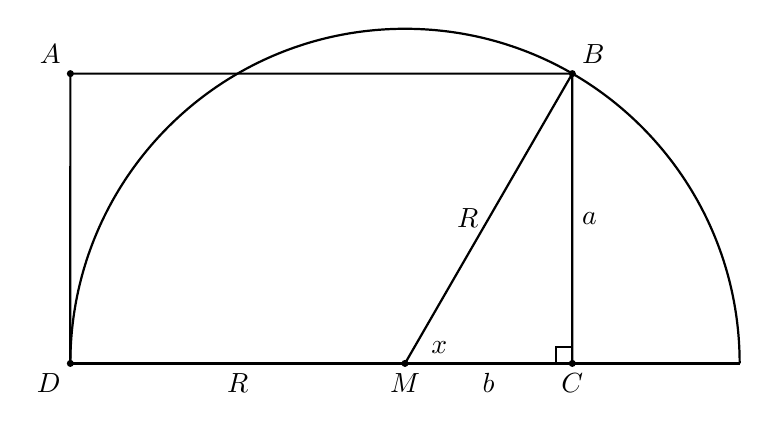
\begin{tikzpicture}[scale=.85]
\coordinate (M) at (0,0);
\coordinate (D) at (-5,0);
\coordinate (B) at (60:5);
\coordinate (A) at (D |- B);
\coordinate (C) at (B |- M);
\draw[thick] (D) arc[start angle=180,end angle=0,radius=5cm];
\draw[thick] (D) -- (A) -- (B) -- (C);
\draw[thick] (-5,0) -- (5,0);
\draw[thick] (M) -- node[left] {$R$} (B);
\fill (A) circle(1.5pt) node[above left] {$A$};
\fill (B) circle(1.5pt) node[above right] {$B$};
\fill (C) circle(1.5pt) node[below] {$C$};
\fill (D) circle(1.5pt) node[below left] {$D$};
\fill (M) circle(1.5pt) node[below] {$M$} node[above right,xshift=6pt] {$x$};
\draw[thick,rotate=90] (C) rectangle +(7pt,7pt);
\path (D) -- node[below] {$R$} (M);
\path (M) -- node[below] {$b$} (C);
\path (C) -- node[right] {$a$} (B);
\end{tikzpicture}
\end{center}

\textbf{סעיף א}

עם הסימונים בתרשים:
\[
S(x)=a(R+b)=R\sin x(R+R\cos x)=R^2\sin x (1+\cos x)\,.
\]
נחשב את הנגזרת:
\erh{2pt}
\begin{equationarray*}{rcl}
S'(x)&=&R^2 (\cos x(1+\cos x) + \sin x \cdot -\sin x)\\
&=&R^2(\cos x + \cos^2 x -\sin^2 x)\\
&=&R^2(\cos x + \cos^2 x -(1-\cos^2 x))\\
&=&R^2(2\cos^2 x+\cos x -1 )=0\\
&=&R^2(2\cos x -1)(\cos x + 1)=0\,.
\end{equationarray*}

\np

אנחנו פוסלים את הפתרון
$\cos x=-1$
כי
$x=180^\circ$
לא יכול להיות זווית במשולש.

לכן,
$\cos x=\frac{1}{2}$, $x=60^\circ$.

הנגזרת השנייה היא:
$(2\cos^2 x+ \cos x -1)'=-\sin x(4\cos x+1)$.
\[
-\sin 60(4\cos 60+1)=-\frac{\sqrt{3}}{2}\cdot (4\cdot\frac{1}{2}+1)=-\frac{3\sqrt{3}}{2}<0\,,
\]
ןלכן נקודת הקיצון היא מקסימום.

\bigskip

\textbf{סעיף ב}

\[
\int_0^{\frac{\pi}{2}} R^2\sin x (1+\cos x) dx = \left. R^2 \cdot -\frac{1}{2}(1+\cos x)^2\right|_0^{\frac{\pi}{2}}=-\frac{R^2}{2}(1^2-2^2)=\frac{3R^2}{2}\,.
\]

\np


%%%%%%%%%%%%%%%%%%%%%%%%%%%%%%%%%%%%%%%%%%%%%%%%%%%%%%%%%%%%%%%%%%%%%%

\section{קיץ תשע"ד מועד א}

\begin{center}
\selectlanguage{english}
\includegraphics[width=\textwidth]{summer-2014a-8}
\end{center}

\vspace{-2ex}

\textbf{סעיף א}

כאשר 
$x$
עולה בערכים חיוביים, הנגזרת עולה בצורה תלולה מערכים שליליים ובצורה מתונה לערכים 
חיוביים, ולכן הפונקציה יורדת בצורה תלולה ואח"כ עולה בצורה מתונה.

כאשר 
$x$
עולה בערכים שליליים, הנגזרת יורדת בצורה מתונה מערכים חיוביים ובצורה תלולה לערכים שליליים, ולכן הפונקציה עולה בצורה מתונה ואח"כ יורדת בצורה תלולה.

לפי התרשים הנתון בנקודה 
$x=-1$
יש נקודה קיצון שהיא מקסימום כי השיפוע יורד. בנקודה 
$x=1$
יש נקודת קיצון שהיא מינימום כי השיפוע עולה. לפי המידע הנתון על הפתרונות של
$f(x)$,
נקודת הקיצון שהיא המקסימום היא 
$(-1,-2)$
ונקודת הקיצון שהיא מינימום היא
$(1,2)$,
כי אם יש רק פתרון אחד, גרף הפונצקיה לא יכול לחצות את הקווים
$y=-2,y=2$.

\begin{center}
\selectlanguage{english}
\begin{tikzpicture}%[scale=.8]
\begin{axis}[
    axis lines=center,
    xmin = -3,
    xmax = 3,
    ymin = -4,
    ymax = 4,
    yticklabel style={anchor=north east,},
]
\addplot [
    domain=-3:-.2,
    samples=50,
]
{x+(1/x)};
\addplot [
    domain=.2:3,
    samples=50,
]
{x+(1/x)};
\draw[dashed,thick] (axis cs:-3,-2) -- (axis cs:3,-2);
\draw[dashed,thick] (axis cs:-3,2) -- (axis cs:3,2);
\fill (axis cs:-1,-2) circle(1.5pt);
\fill (axis cs:1,2) circle(1.5pt);
\end{axis}
\end{tikzpicture}
\end{center}

\np

\textbf{סעיף ב}

לפי הגרף
$f'(1)=f'(-1)=0$
ונתון 
$a\neq 0$,
ולכן
$\disfrac{a-b}{a}=0$,
ו-%
$a=b$.

שוב בגלל ש-%
$a\neq 0$
אפשר לצמצם את הפרמטרים:
\[
f'(x)=\frac{a(x^2-1)}{ax^2}=\frac{x^2-1}{x^2}\,.
\]
נחשב את האיטרגל של הנגזרת כדי למצוא את הפונקציה:
\[
f(x)=\int f'(x)\, dx = \int \left(1-\frac{1}{x^2}\right)dx = x+\frac{1}{x}+c\,.
\]
הנגזרת מתאפסת ב-%
$\pm 1$,
ולכן נקודות המינימום והמקסימום גם הן ב-%
$\pm 1$:
\erh{10pt}
\begin{equationarray*}{rcl}
1+\frac{1}{1}+c&=&2\\
-1+\frac{1}{-1}+c&=&-2\,,
\end{equationarray*}
ולכן
$c=0$.

הפונקציה היא
$f(x)=x+\disfrac{1}{x}$.

\np


%%%%%%%%%%%%%%%%%%%%%%%%%%%%%%%%%%%%%%%%%%%%%%%%%%%%%%%%%%%%%%%%%%%%%%

\section{חורף תשע"ד}

\begin{center}
\selectlanguage{english}
\includegraphics[width=.85\textwidth]{winter-2014-9}
\end{center}

\vspace{-2ex}

\textbf{בבחינה זו היו שלוש שאלות בפרק השני לכן מספר השאלה הוא 
$9$
ולא 
$8$.}

\textbf{סעיף א}

לפי הטבלה הפונקציה עולה מ-%
$x=1.1$
דרך 
$x=1.2$
ל-%
$x=1.3$.
נתון שאין נקודות קיצון פנימיות ולכן הנגזרת הראשונה חיובית.

\textbf{סעיף ב}

הנגזרת השנייה שלילית כך שהנגזרת הראשונה יורדת בתחום ולכן הטענה נכונה.

\textbf{סעיף ג}

\[
g'(x)=\frac{1}{2} f(x)^{-\frac{1}{2}} f'(x)\,.
\]
מסעיף א, גם 
$f(x)$
וגם
$f'(x)$
חיוביים בתחום, ולכן 
$g'(x)$
חיובי, ו-%
$g(x)$
עולה בתחום.

\textbf{סעיף ד}
\erh{12pt}
\begin{equationarray*}{rcl}
g'(x) &=& f'(x)\\
\frac{1}{2\sqrt{f(x)}} f'(x) &=& f'(x)\\
f(x)&=&\frac{1}{4}\,.
\end{equationarray*}
מצאנו שהנגזרת הראשונה חיובית כך שאפשר לצמצם אותה. לפי הטבלה,
$f(x)$
איננה פונקציה קבועה בכל התחום, לכן לא ייתכן ש-%
$g'(x) = f'(x)$.

\selectlanguage{english}
